\documentclass{article}
\usepackage{graphicx}
\usepackage[top=1in, bottom=1in, left=1in, right=1in]{geometry}

\begin{document}

\title{Text Technologies for Data Science: Assessment 2}
\author{s1107496}

\maketitle

\section{Introduction}
This report describes the implementation of two information retrieval algorithms, brute.py and index.py, as well as refinements to the latter as implemented in best.py.

\section{brute.py and best.py}
\subsection{brute.py}
In overlap.py, each query and document was first transformed to lowercase and tokenized, with tokens matching the simple regular expression \texttt{[A-Za-z0-9]+}. For every combination of document and query, the score returned was the size of the intersection of the token sets for the document and query. This method resulted in an average precision of 0.1527.
\subsection{tfidf.py}
tfidf.py implemented the standard tf-idf algorithm, with k=2 and using the natural logarithm. For speed, df-scores for each token were pre-calculated. The tf-idf algorithm resulted in an average precision of 0.3248.

\section{best.py}
best.py included a number of refinements over tfidf.py, as listed below. The average precision achieved by best.py was 0.3508.
\subsection{Stop word removal}
After initial tokenization using the same regular expression as overlap.py, all tokens from the English-language stop word list provided by \texttt{nltk} were removed. This was performed for both queries and documents, and increased average precision by 0.0088.
\subsection{Character n-grams}
To account for morphological variation, each token was broken into constituent n-grams, which were then themselves added to the token list. This procedure was performed for both queries and documents. As stated in the 29th September, 2014 Text Technologies lecture, character n-grams of length 4 or 5 work best for European languages - in this case, 4-grams yielded an average precision advantage of 0.003 over 5-grams. Adding both 4- and 5-grams decreased average precision. Overall, this method increased average precision by 0.0066.
\subsection{Bigrams}
In both documents and queries, to capture meaningful pairings of words, bigrams from the stop-word-sanitized token list were themselves added to the token list. This improved average precision by 0.0033, and was found to be more effective than trigrams or both bigrams and trigrams.
\subsection{Extended token set}
For both documents and queries, the text was additionally tokenized via the regex \texttt{[A-Za-z0-9\symbol{92}.\symbol{92}-\symbol{92}\_\symbol{92}/]+}, which preserves e.g. the tokens "I.B.M." and "n-tuples". These extended tokens were then added to the token list, if not already present, with all punctuation intact. This resulted in a precision increase of 0.0022.
\subsection{\texttt{k} optimization}
The value of \texttt{k} within the standard formulation of tf-idf was hand-optimized to a value of 3.0, yielding a 0.0051 increase in average precision. The figure below demonstrates the observed effect of k on precision.
%\begin{figure}[ht!]
%\centering
%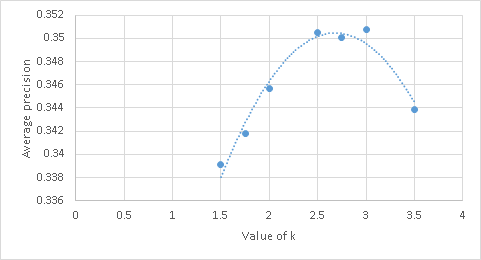
\includegraphics[width=90mm]{k_graph2.png}
%\end{figure}
\subsection{Unsuccessful techniques}
The following techniques were implemented, but uniformly had a negative effect on average precision and, hence, were discarded:
\begin{itemize}
\item Weighting references - A scheme whereby documents had their tf-idf score slightly increased   proportionally to the scores of all documents that referenced them reduced average precision to 0.1949.
\item Synonymy - For each token, synonyms of that token were calculated via the Expected Mutual Information Measure as presented in the Text Technologies lecture on 29th September 2014. Tokens were considered synonymous when the EMIM of the two terms was 2 standard deviations above the average. For performance reasons, EMIM was only calculated for tokens appearing in 10\%-0.67\% of documents. For each query, all tokens with synonyms had their synonyms added to the token list. Overall, this led to a .0090 reduction in average precision, with a significant increase in computation time.
\end{itemize}

\end{document}